\textbf{مورد استفاده:}
واگذاری پروژه
\\
\textbf{شرح مختصر :UC}
در این قسمت کارفرما پروژه را به یک فریلنسر واگذار می‌کند.
\\
\textbf{پيش شرط:}
ورود به مدیریت پروژه در داشبورد کارفرما.
\\
\textbf{سناريو اصلی:}
\begin{enumerate}
\item
شروع
\item
کارفرما دکمه قرارداد پروژه را انتخاب می‌کند و سیستم پیشنهادات فریلنسرها را به کارفرما نمایش می‌دهد.
\item
کارفرما بهترین پیشنهاد را انتخاب می‌کند و با دکمه تایید قرارداد را مشاهده کرده و وضعیت پیشنهاد را به سیستم ارسال می‌کند.
\item
سیستم به فریلنسر اطلاع داده و در بانک اطلاعات ثبت می‌کند.
\item
پایان
\end{enumerate}

\noindent
\textbf{پس شرط:}
فریلنسر باید برای ادامه قرارداد را تایید کند.
\\
\textbf{سناريوهای فرعی:}
ندارد.
\\
\textbf{پس شرط:}
ندارد.



\begin{figure}[H]
	\centering
	\includegraphics[width=.8\textwidth]{Diagram/2.Activity/کارفرما/مدیریت-پروژه-قرارداد-تایید.png}
	\caption{دیاگرام فعالیت واگذاری پروژه}
	\label{fig:a:واگذاری-پروژه}
\end{figure}
\begin{figure}[H]
\centering
\includegraphics[width=.8\textwidth]{Diagram/3.StateMachine/کارفرما/مدیریت-پروژه-قرارداد-تایید.png}
\caption{دیاگرام حالت ماشین واگذاری پروژه}
\label{fig:sm:واگذاری-پروژه}
\end{figure}
\begin{figure}[H]
	\centering
	\includegraphics[width=1\textwidth]{Diagram/4.Collaboration/1.Sequence/کارفرما/مدیریت-پروژه-قرارداد-تایید.png}
	\caption{دیاگرام توالی واگذاری پروژه}
	\label{fig:s:واگذاری-پروژه}
\end{figure}
\begin{figure}[H]
\centering
\includegraphics[width=0.7\textwidth]{Diagram/4.Collaboration/2.Communication/کارفرما/مدیریت-پروژه-قرارداد-تایید.png}
\caption{دیاگرام همکار واگذاری پروژه}
\label{fig:c:واگذاری-پروژه}
\end{figure}
